\section{Разработка интеллектуальной справочной системы по библиографии}
\label{sec:development}

Ниже представены фрагменты из базы знаний интеллектуальной справочной системы по библиографии, а именно предметной области японского литературного направления.

\subsection{Примеры описания разделов}

Рисунок \ref{fig:fragment_japanese_literature} представляет собой фрагмент базы знаний интеллектуальной справочной системы, специализированной по библиографии японского литературного направления, а также соотвеcтвующая сущность предметной области. На изображении отражены ключевые sc-элементы, связанные с областью исследования, декомпозиция раздела для обеспечения удобного и систематического представления информации. Помимо этого, представлена исследуемые в предметной области японского литературного направления отношения.

\begin{figure}[H]
    \centering
    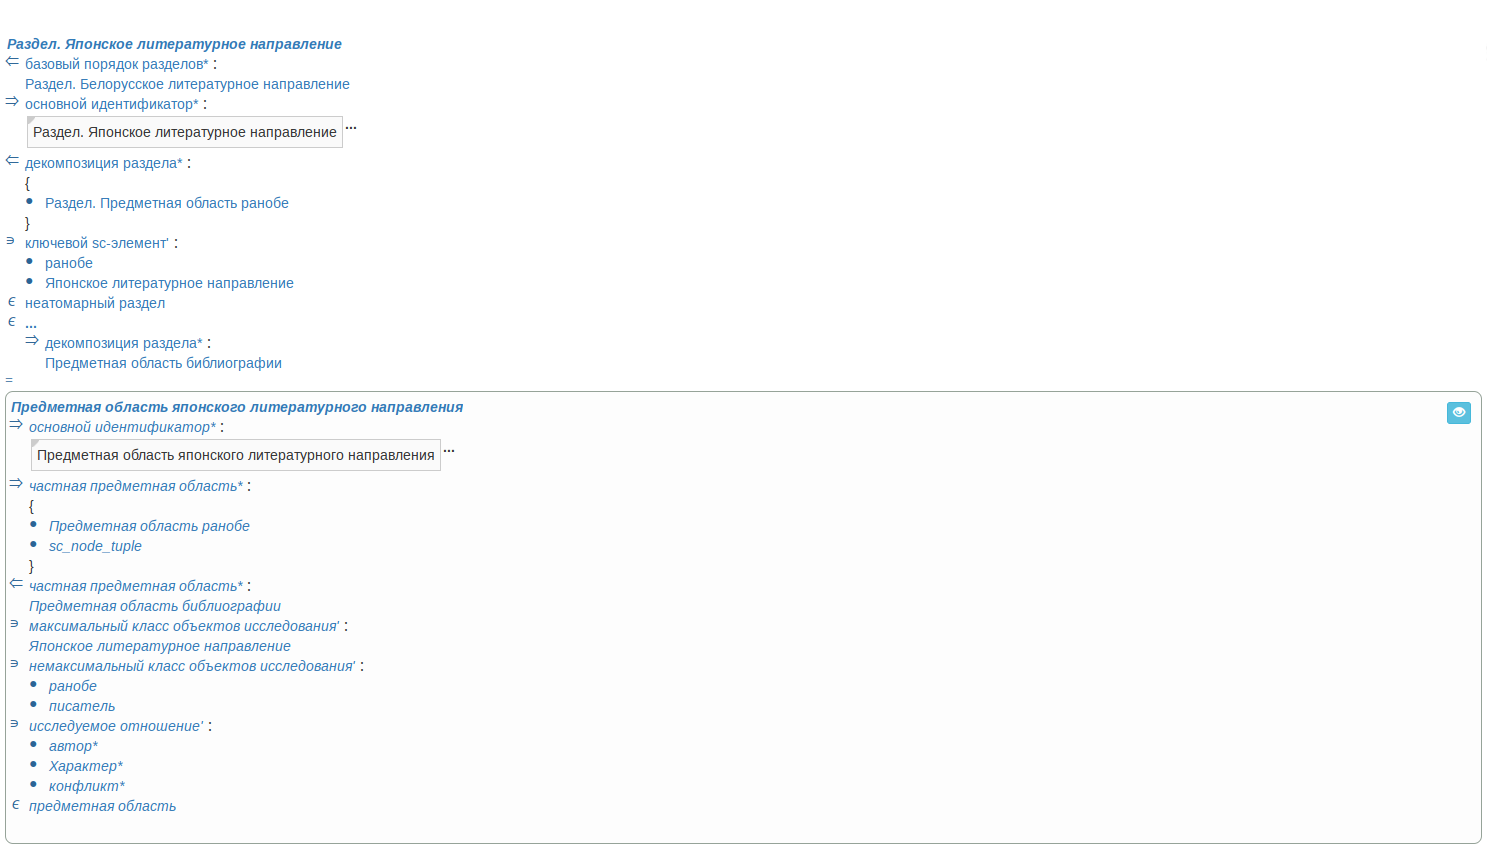
\includegraphics[scale=0.41]{imgs/japanese_literature.png}
    \caption{Фрагмент базы знаний интеллектуальной справочной системы по библиографии: Раздел. Японское литературное направление}
    \label{fig:fragment_japanese_literature}
\end{figure}

Рисунок \ref{fig:subj_ranobe} представляет собой фрагмент, описывающий раздел и предметную область ранобе, конкретного направления в японсккой литературе, их декомпозицию (авторы ранобе, иллюстраторы ранобе, сами ранобе, концепции, популярные в ранобе, жанры ранобе), исследуемые отношения, объекты исследования.

\begin{figure}[H]
    \centering
    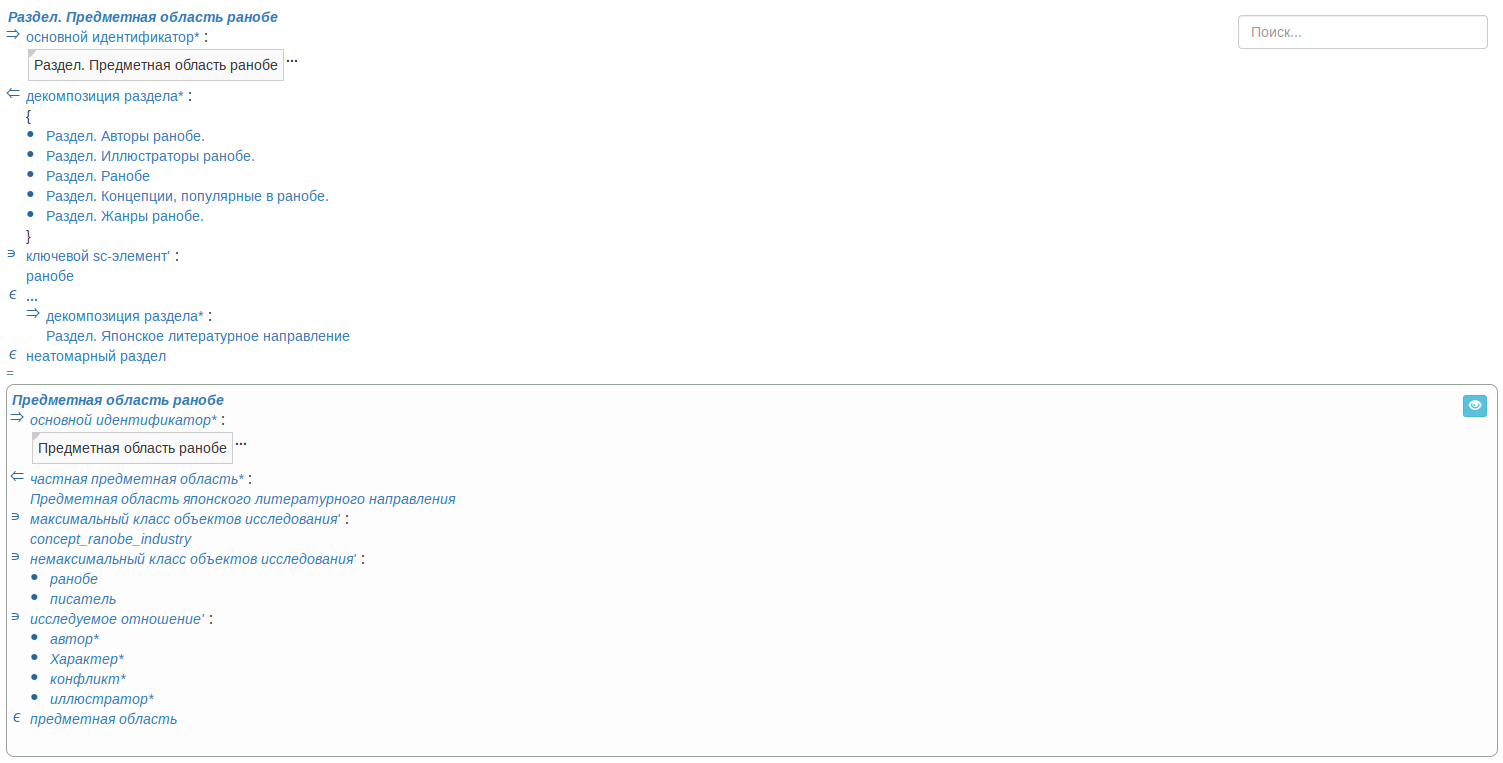
\includegraphics[scale=0.4]{imgs/subj_ranobe.png}
    \caption{Фрагмент базы знаний интеллектуальной справочной системы по библиографии: Раздел. Предметная область ранобе}
    \label{fig:subj_ranobe}
\end{figure}

\subsection{Примеры описания абсолютных понятий}

% Количество абсолютных понятий доминирует над количеством относительных понятий в базах знаний интеллектуальной справочной системы по библиографии. На рисунке \ref{fig:absolute_ranobe} представлен пример абсолютного понятия "ранобе", где приведено его определение на естественном языке, указаны предметные области, объектами исследования которых является данная сущность, утверждения, в которых используется данная сущность и сущности, являющиеся элементами множества ранобе.

На рисунке \ref{fig:absolute_ranobe} представлен пример абсолютного понятия <<ранобе>>, где приведено его определение на естественном языке, указаны предметные области, объектами исследования которых является данная сущность, утверждения, в которых используется данная сущность и сущности, являющиеся элементами множества ранобе.

\begin{figure}[H]
    \centering
    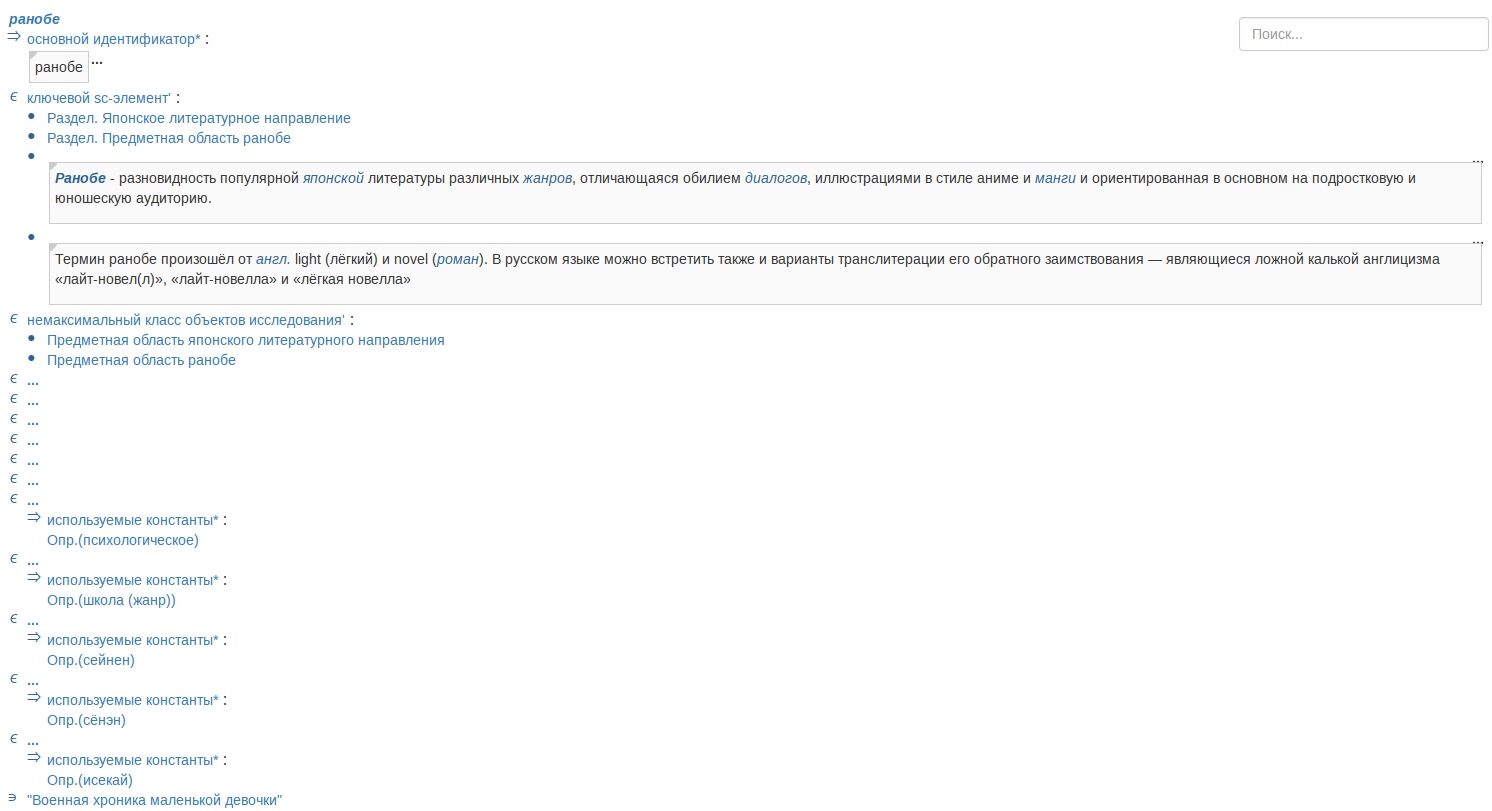
\includegraphics[scale=0.415]{imgs/ranobe.png}
    \caption{Фрагмент базы знаний интеллектуальной справочной системы по библиографии: абсолютное понятие "ранобе"}
    \label{fig:absolute_ranobe}
\end{figure}

На рисунке \ref{fig:section_genres} показан раздел, описывающий жанры, специфичные для ранобе, их описание на естественном языке, элементы множества этого жанра, место жанра в иерархии сущностей базы знаний.

\begin{figure}[H]
    \centering
    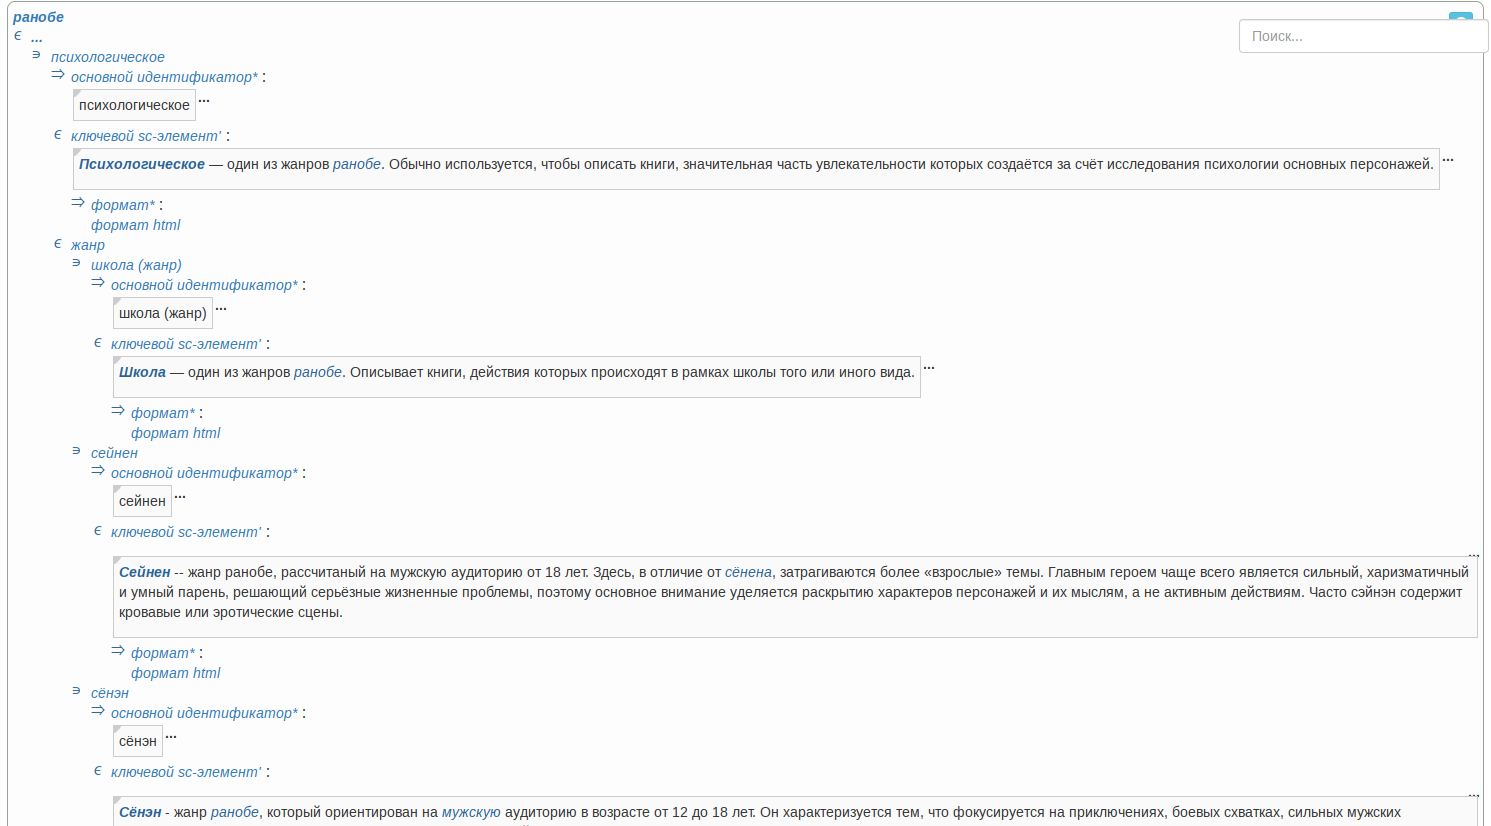
\includegraphics[scale=0.41,trim={0 5cm 0 0},clip]{imgs/genres.png}
    \caption{Фрагмент базы знаний интеллектуальной справочной системы по библиографии: Раздел. Жанры ранобе}
    \label{fig:section_genres}
\end{figure}

%На рисунке \ref{fig:section_genres} приведён пример оформления раздела, описывающего жанры, специфичные для ранобе. Присутствует описание на естественном языке, элементы множества, соответствующие этому жанру, место жанра в иерархии сущностей базы знаний интеллектуальной справочной системы по библиографии.

Раздел на рисунке \ref{fig:authors} содержит информацию об авторах ранобе, включенных в базу знаний интеллектуальной системы, для каждого из которых указано место рождения, язык написания произведений, а также список произведений за их авторством.

\begin{figure}[H]
    \centering
    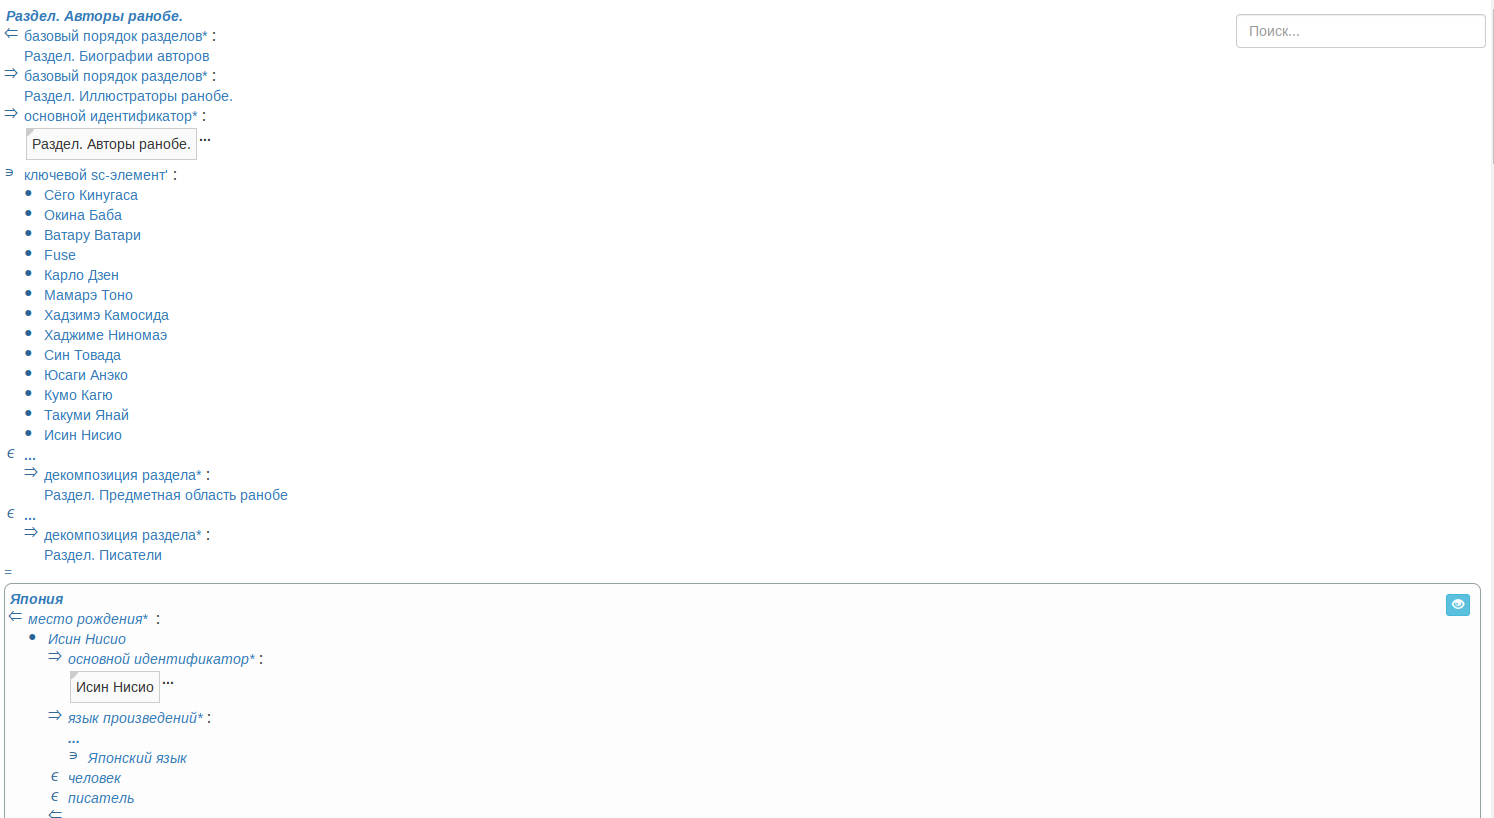
\includegraphics[scale=0.4]{imgs/authors.png}
    \caption{Фрагмент базы знаний интеллектуальной справочной системы по библиографии: Раздел. Авторы ранобе}
    \label{fig:authors}
\end{figure}

\subsection{Примеры описания относительных понятий}

Хоть и большая часть базы знаний является пространством абсолютных понятий, но для описания связей между классами объектов нужны относительные понятия. Так, на рисунке \ref{fig:nrel_illustrator} представлено новое введенное бинарное отношение "иллюстратор*". Для отношения заданы первый и второй домен, приведено определение на естественном языке, определены характеристики данного отношения, такие как арность, ориентированность, асимметричность, антитранзитивность, а также связываемые им сущности.

%Для описания связей между сущностями нужны относительные понятия. Так, на рисунке \ref{fig:nrel_illustrator} представлено новое введенное отношение "иллюстратор*". Для него приведены домены, определение на естественном языке, характеристики, а также связываемые им сущности.

\begin{figure}[H]
    \centering
    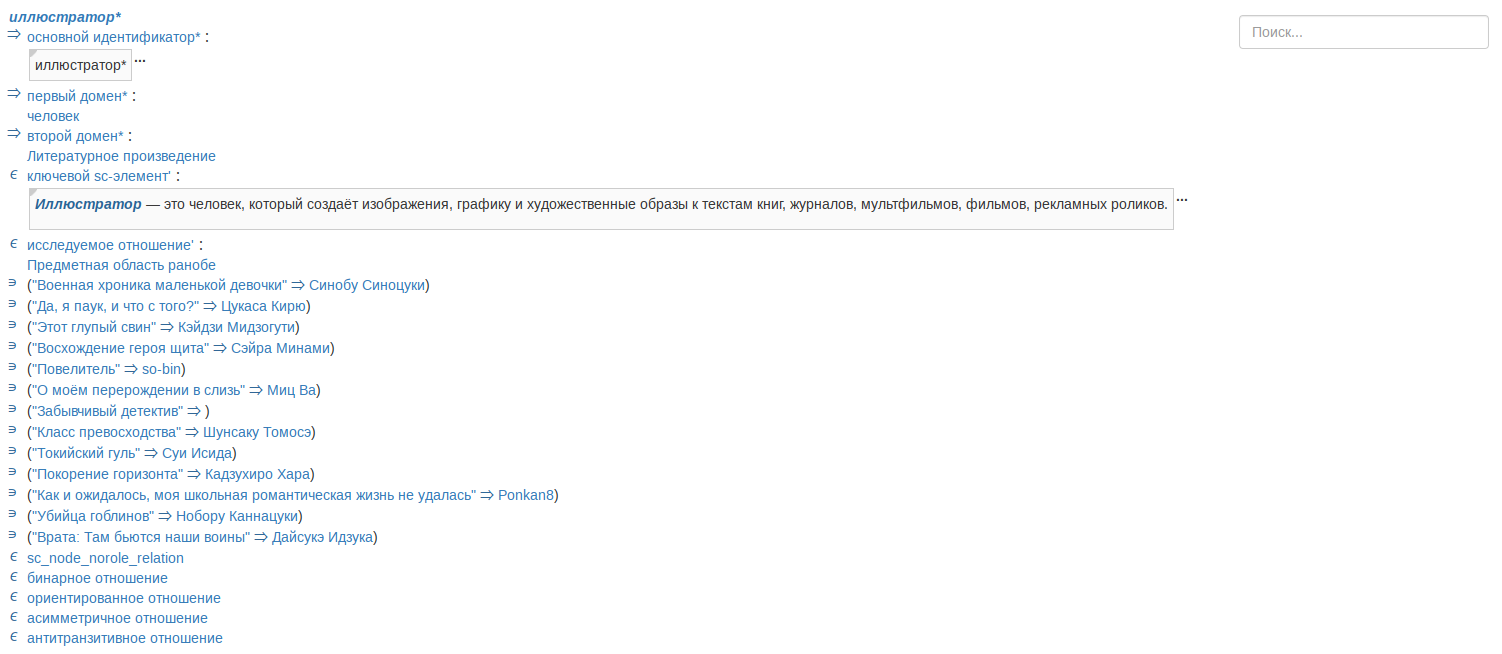
\includegraphics[scale=0.42]{imgs/nrel_illustrator.png}
    \caption{Фрагмент базы знаний интеллектуальной справочной системы по библиографии: отношение "иллюстратор*"}
    \label{fig:nrel_illustrator}
\end{figure}

\subsection{Конкретные сущности}

Отдельное внимание было уделено включению в базу знаний конкретных сущностей -- самих ранобе. На рисунке \ref{fig:overlord} приведён фрагмент базы знаний, содержащий информацию о ранобе "Повелитель". Для него, так же, как и для других формализованных ранобе указаны:
\begin{itemize}
    \item автор произведения
    \item иллюстратор произведения (отличительной чертой ранобе является обязательное наличие иллюстраций)
    \item язык написания оригинала
    \item обложка оригинального издания
    \item список главных и побочных персонажей произведения
    \item подробное описание на естественном языке
    \item жанровая принадлежность
\end{itemize}

\begin{figure}[H]
    \centering
    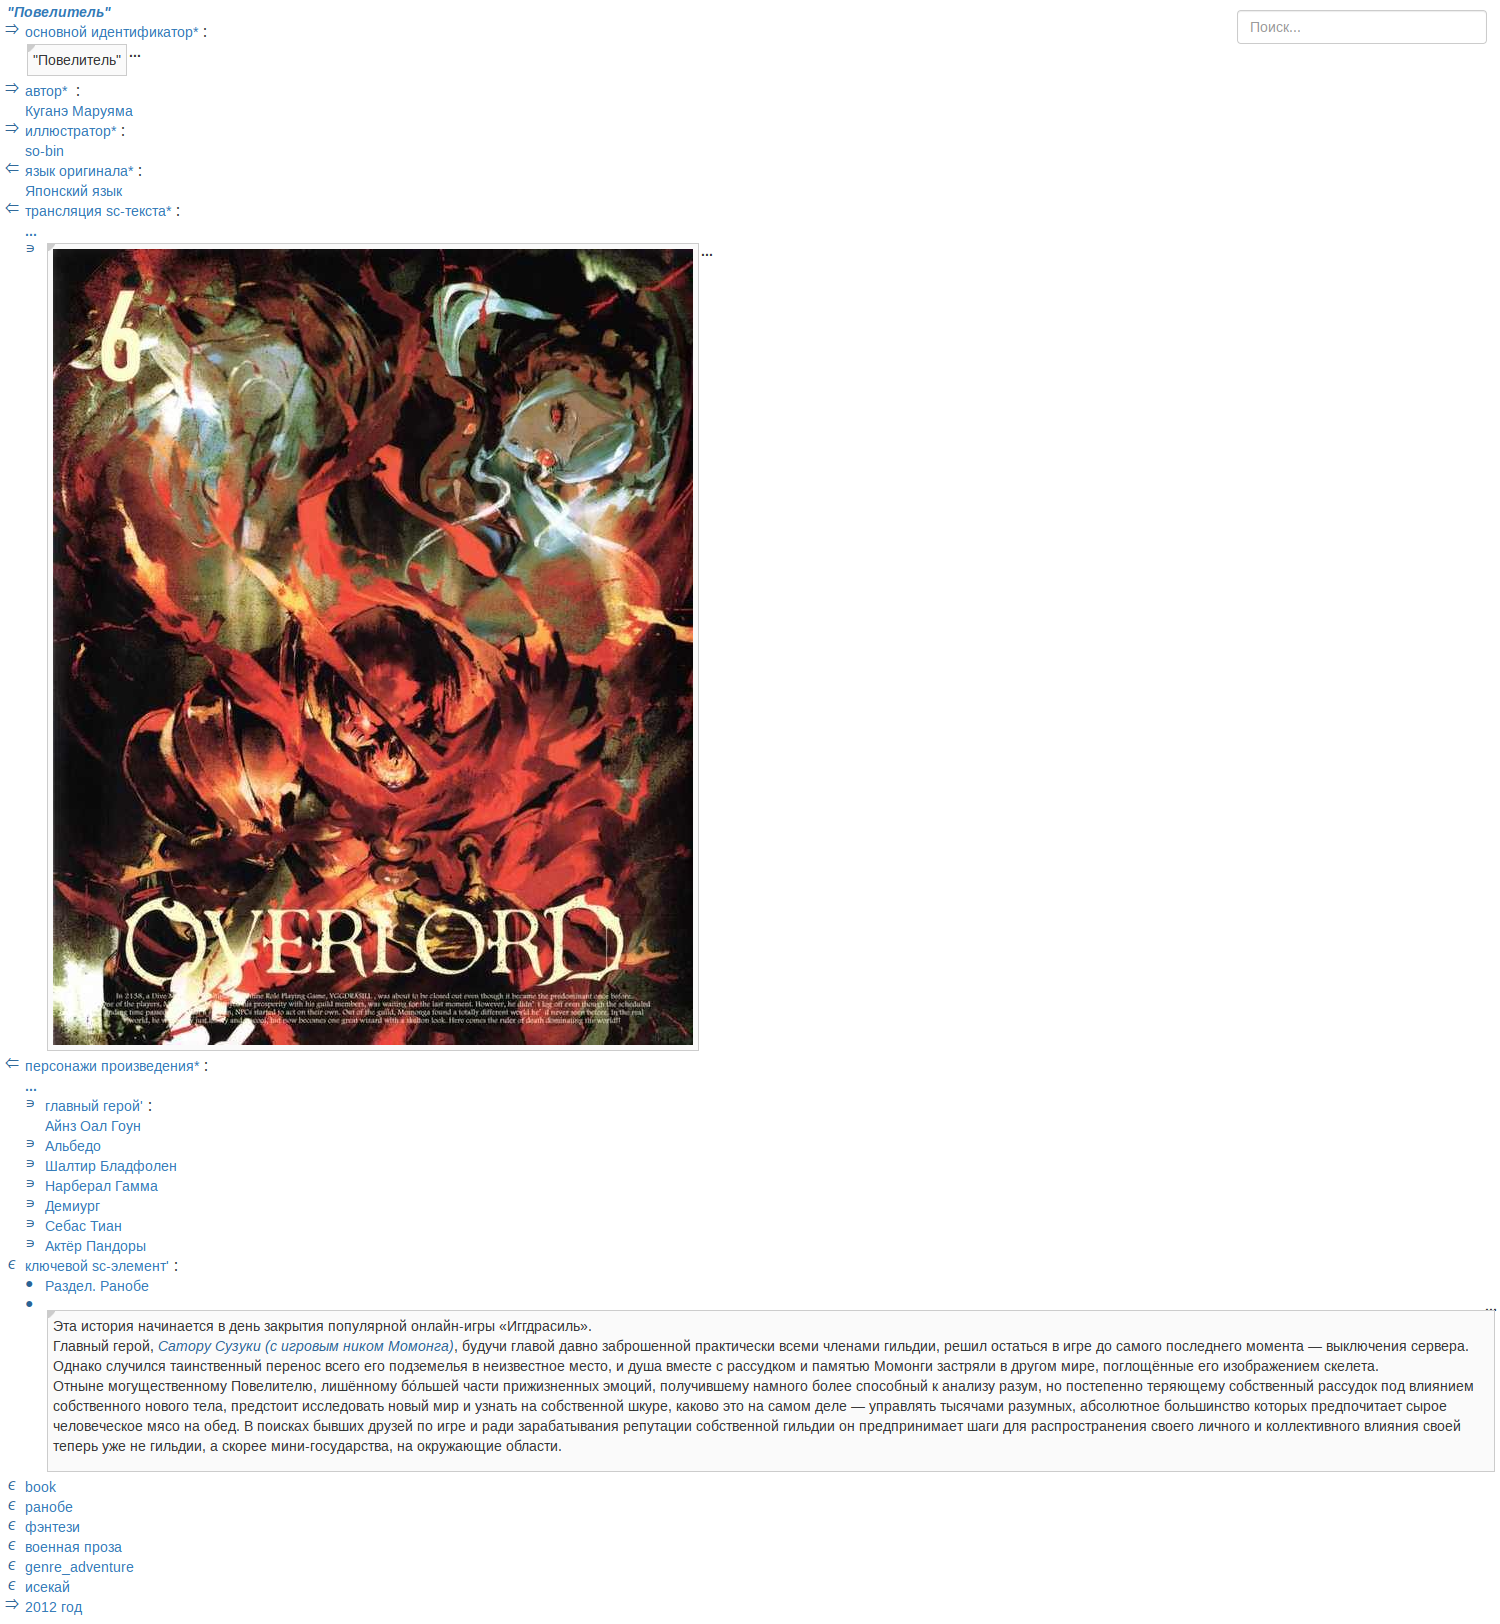
\includegraphics[scale=0.41]{imgs/overlord.png}
    \caption{Фрагмент базы знаний интеллектуальной справочной системы по библиографии: ранобе "Повелитель"}
    \label{fig:overlord}
\end{figure}

Как видно из рисунка выше, в базу знаний также включены сущности персонажей произведений. Пример такого фрагмента приведён на рисунке \ref{fig:character_example}, для каждого персонажа в базу знаний интеллектуальной системы были включены его подробное описание на естественном языке, изображение персонажа, его принадлежность к произведению (произведениям), пол, а также расовая принадлежность (в аниме, манге и ранобе, развивавшимся под большим влиянием жанра фэнтези, нередко встречаются персонажи-нелюди, такие как эльфы, зверолюди, демоны и иные).

\begin{figure}[H]
    \centering
    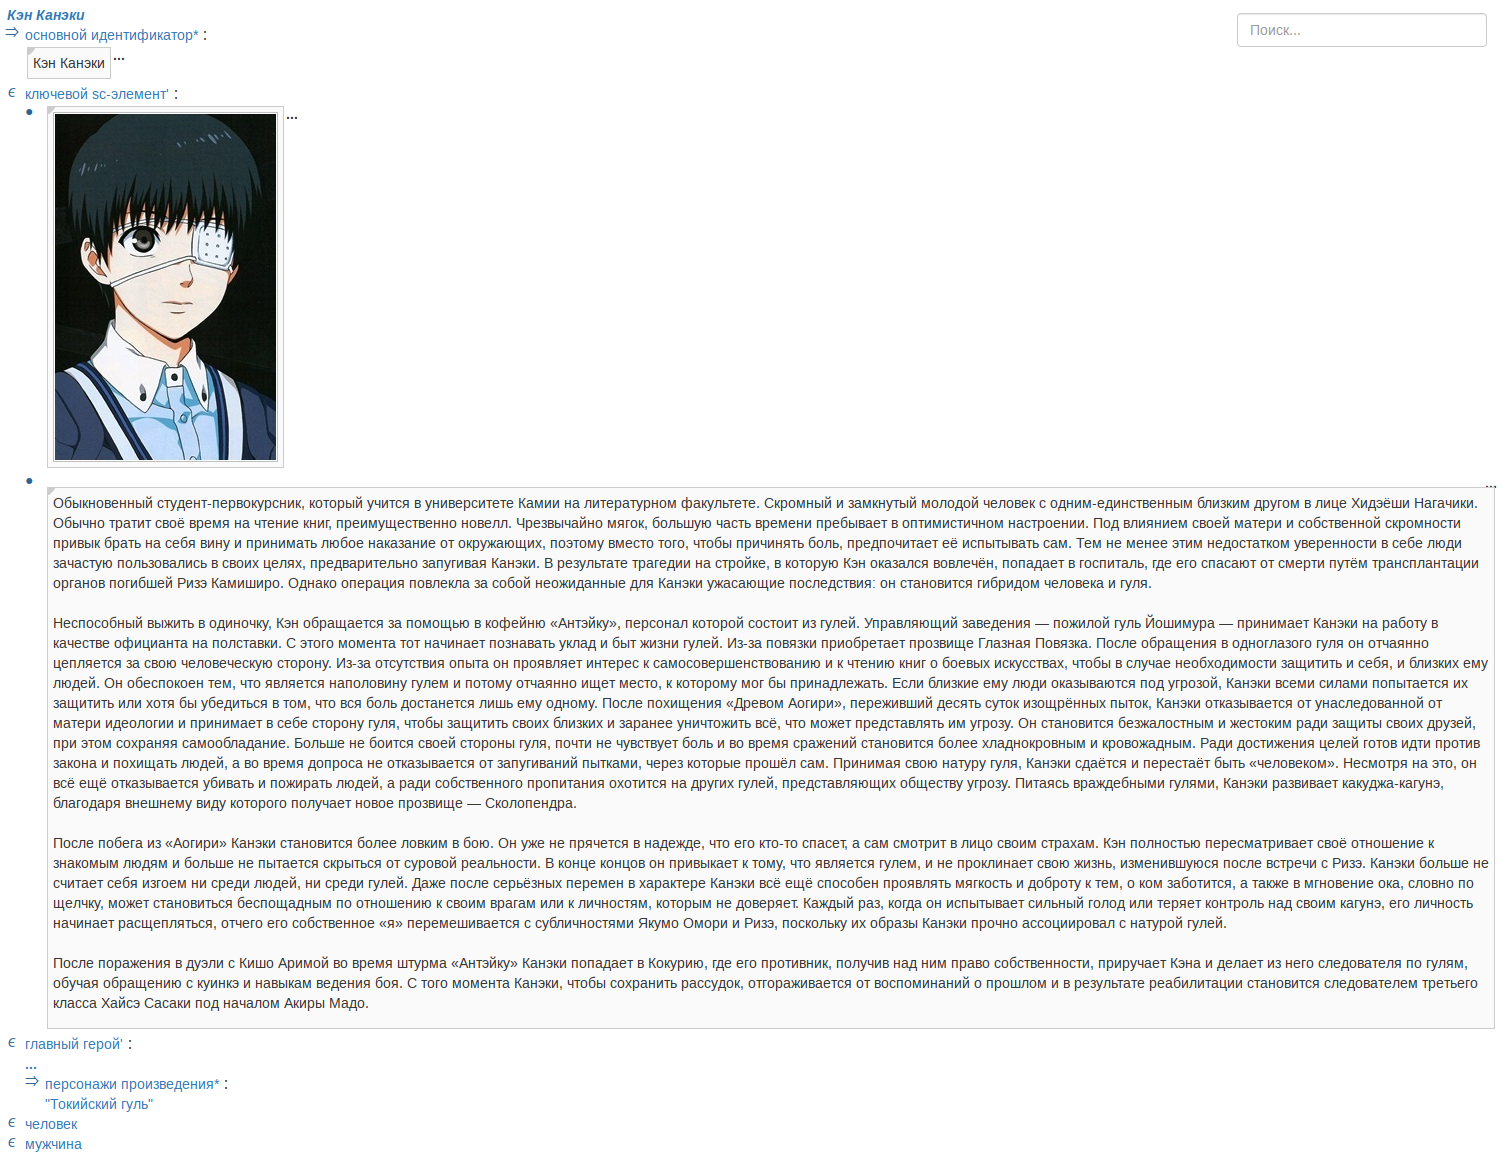
\includegraphics[scale=0.37]{imgs/character_example.png}
    \caption{Пример формализации персонажа в базе знаний интеллектуальной справочной системы по библиографии}
    \label{fig:character_example}
\end{figure}

\subsection{Тестирование базы знаний}

Тестирование базы знаний является важным шагом в разработке интеллектуальных систем, поскольку позволяет проверить ее работоспособность и соответствие требованиям и ожиданиям пользователей. Рассмотрим несколько запросов к системе:

На рисунке \ref{fig:search_isekai} слева изображен запрос для поиска всех ранобе жанра исекай в базе знаний (сущностей, принадлежащих множествам ранобе и исекай), справа результат работы данного запроса в системе.

\begin{figure}[H]
    \centering
    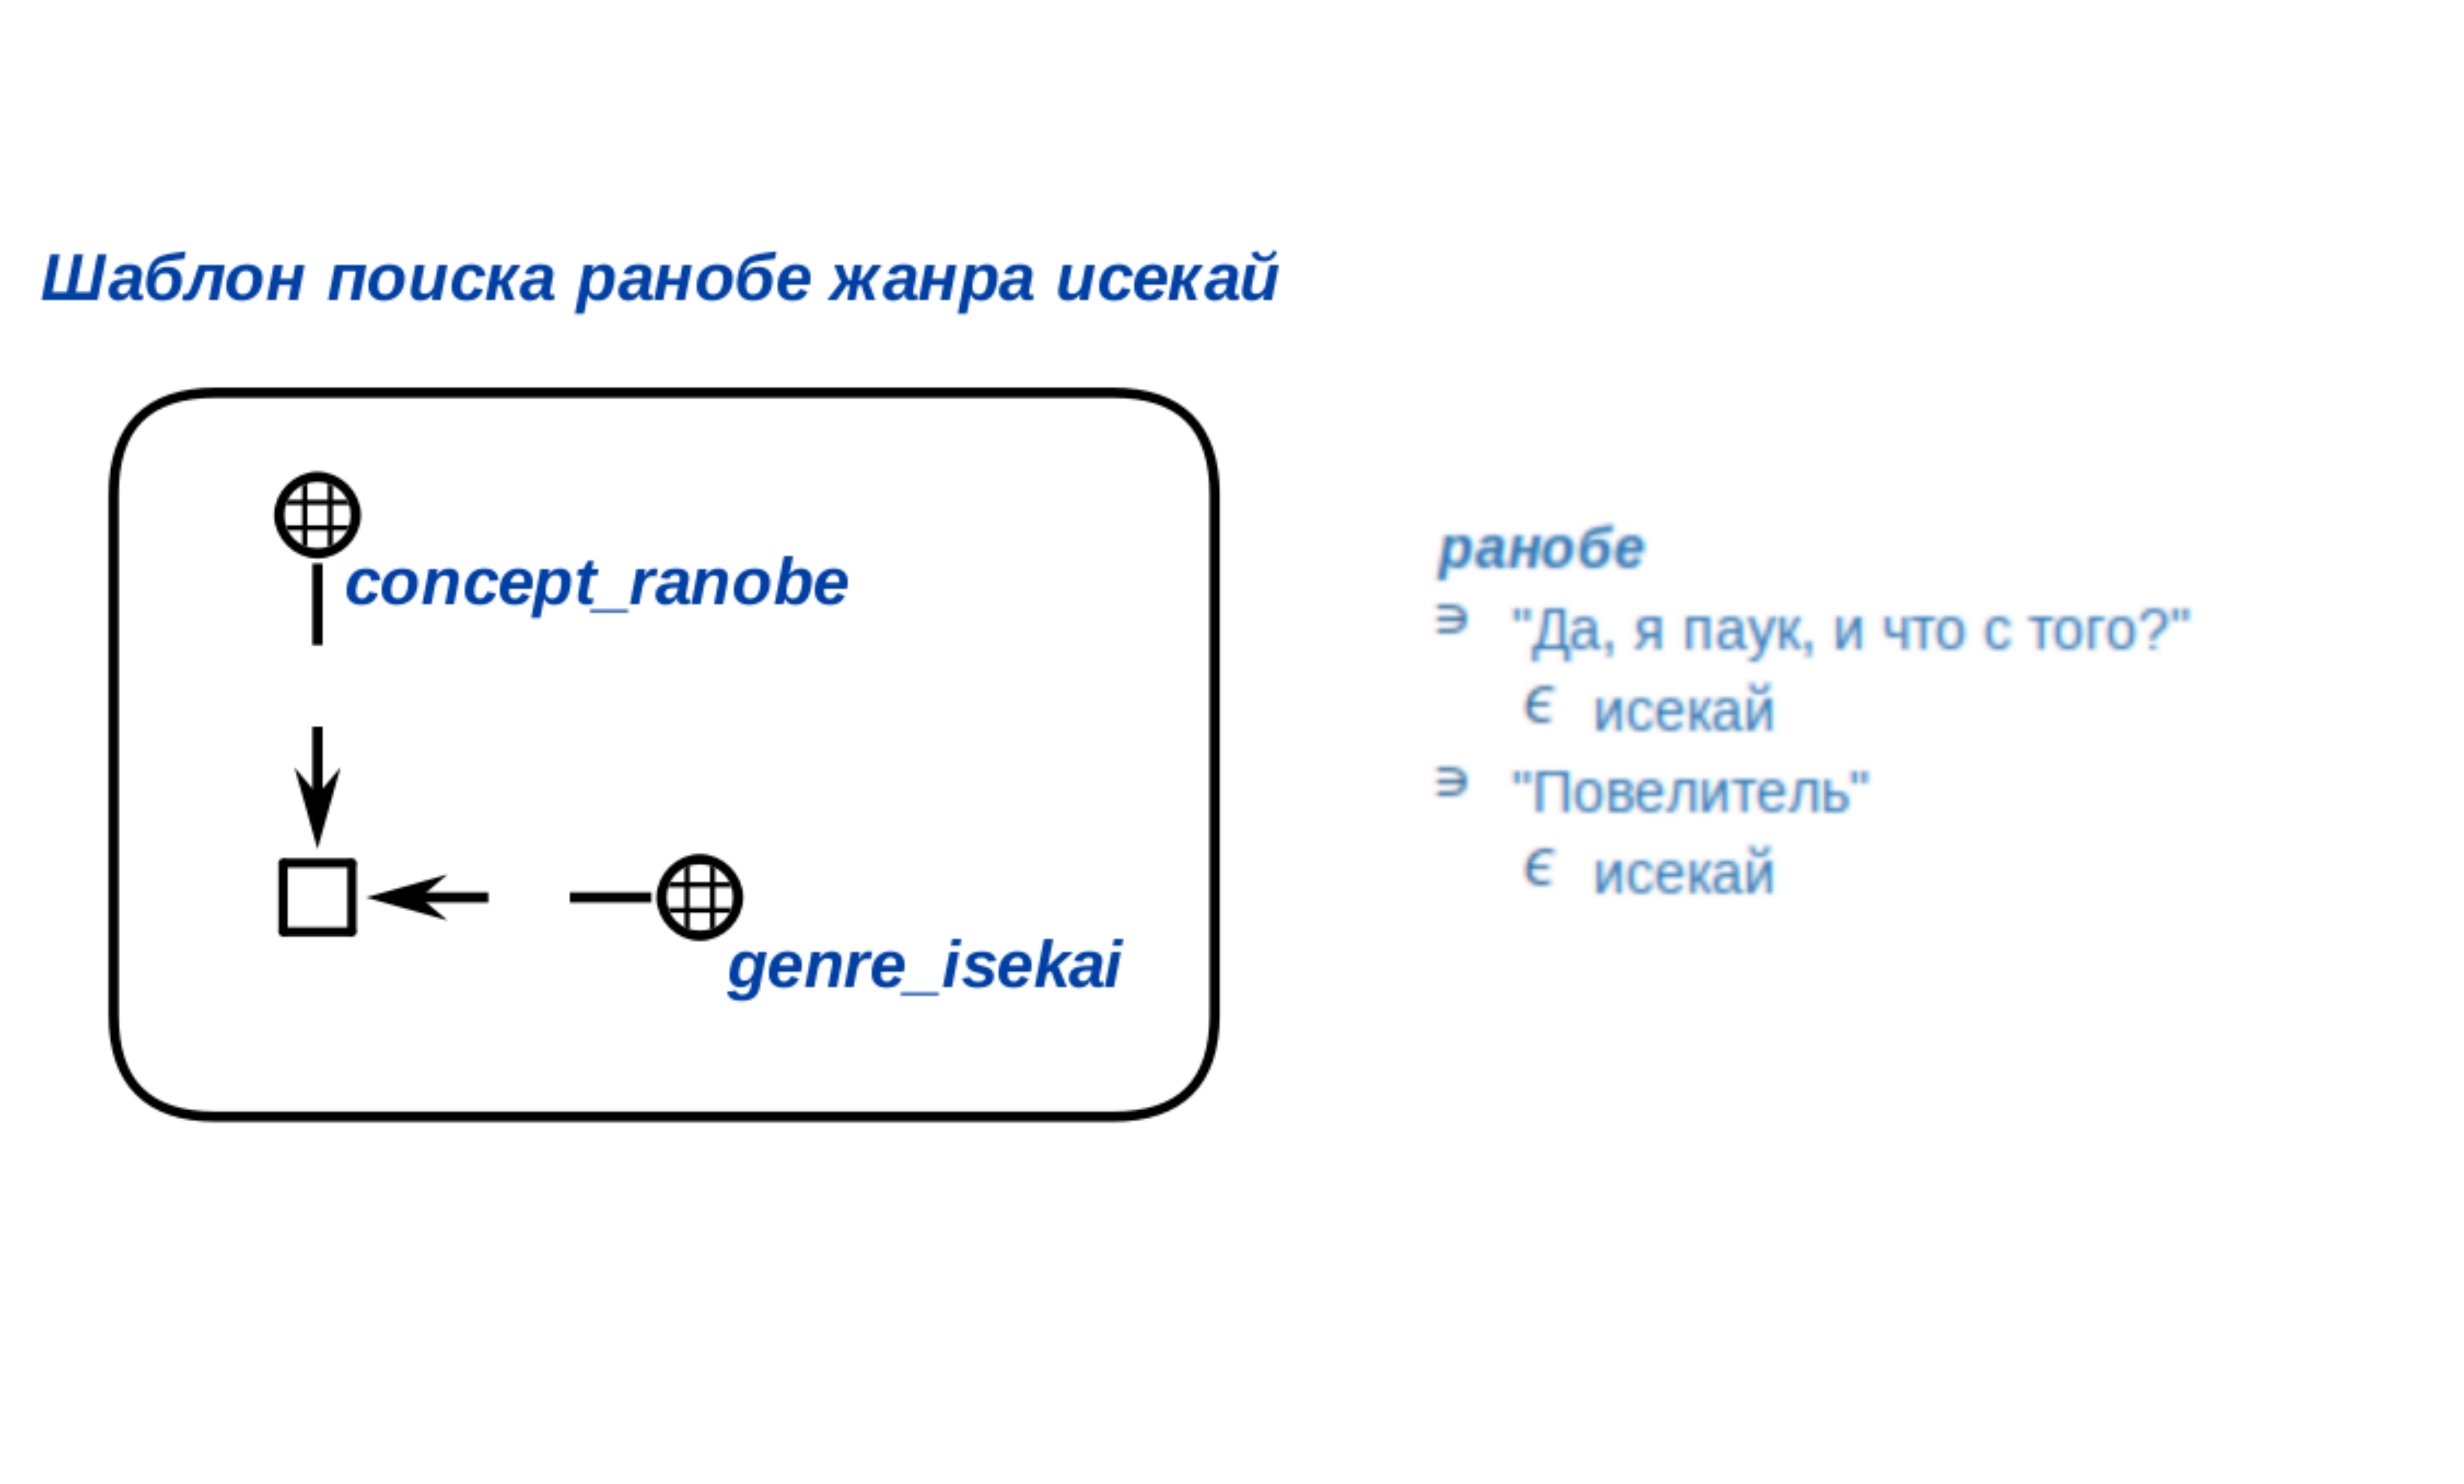
\includegraphics[scale=0.13,trim={0 15cm 0cm 15cm},clip]{imgs/isekai_ranobe_qr.png}
    \caption{Запрос и результат поиска всех ранобе жанра исекай}
    \label{fig:search_isekai}
\end{figure}

На рисунке \ref{fig:search_kumo_kagyu} слева изображен запрос для нахождения автора ранобе, персонажем которого является Убийца Гоблинов (сущности, находящейся в отношении автор* с сущностью, находящейся в отношении персонажи произведения* с сущностью, которой принадлежит персонаж Убийца Гоблинов), справа изображен результат работы данного запроса в системе.

\begin{figure}[H]
    \centering
    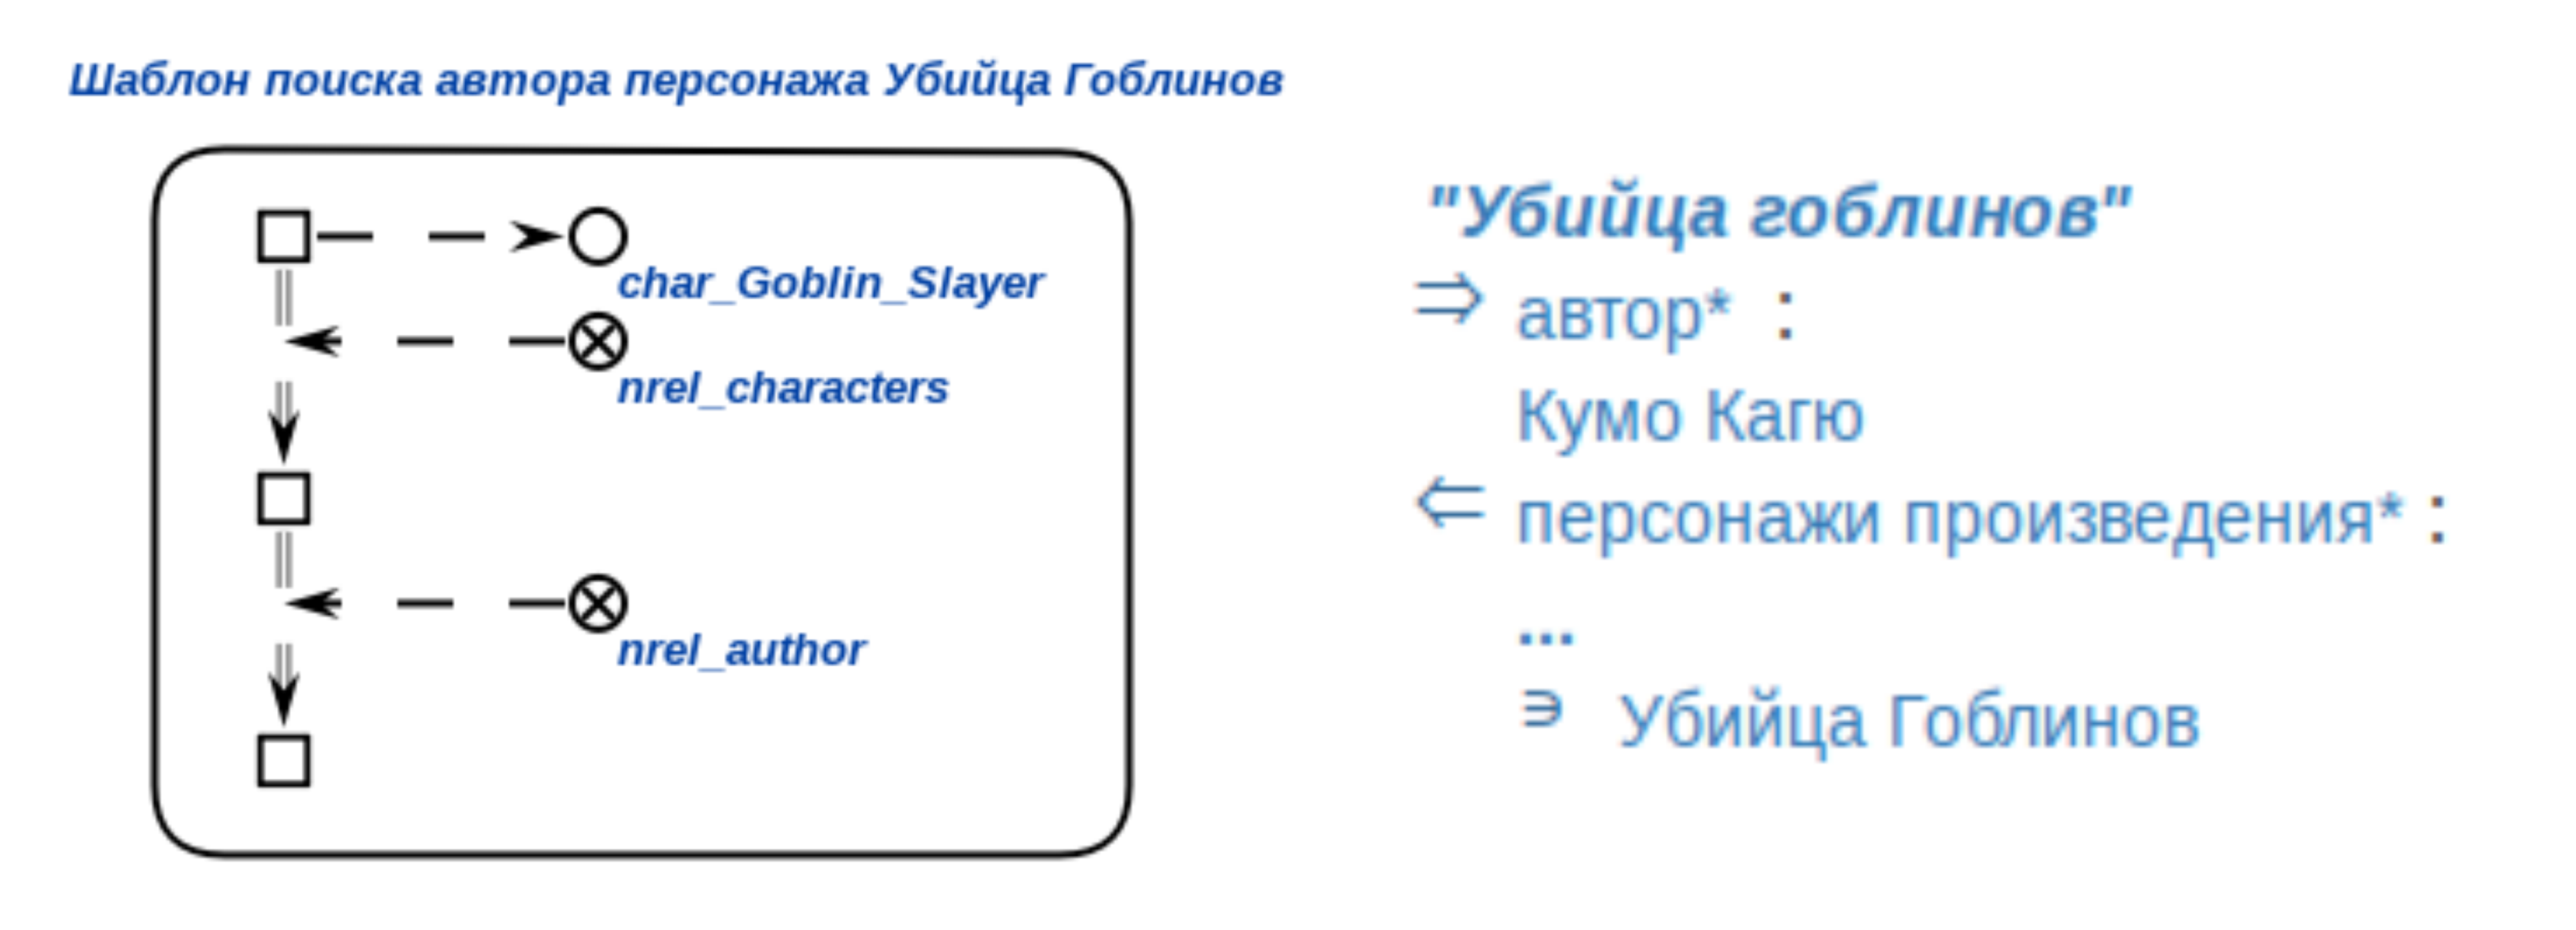
\includegraphics[scale=0.13]{imgs/gs_author_qr.png}
    \caption{Запрос и результат поиска автора ранобе, персонажем которого является Убийца Гоблинов}
    \label{fig:search_kumo_kagyu}
\end{figure}

На рисунке \ref{fig:search_same_genres} слева изображен запрос для нахождения ранобе, имеющих общие жанры с Восхождением Героя Щита (сущностей, принадлежащих множеству ранобе, а также принадлежащих множеству, которые является элементом множества жанров, и которому принадлежит Восхождение Героя Щита), справа изображен результат работы данного запроса в системе.

\begin{figure}[H]
    \centering
    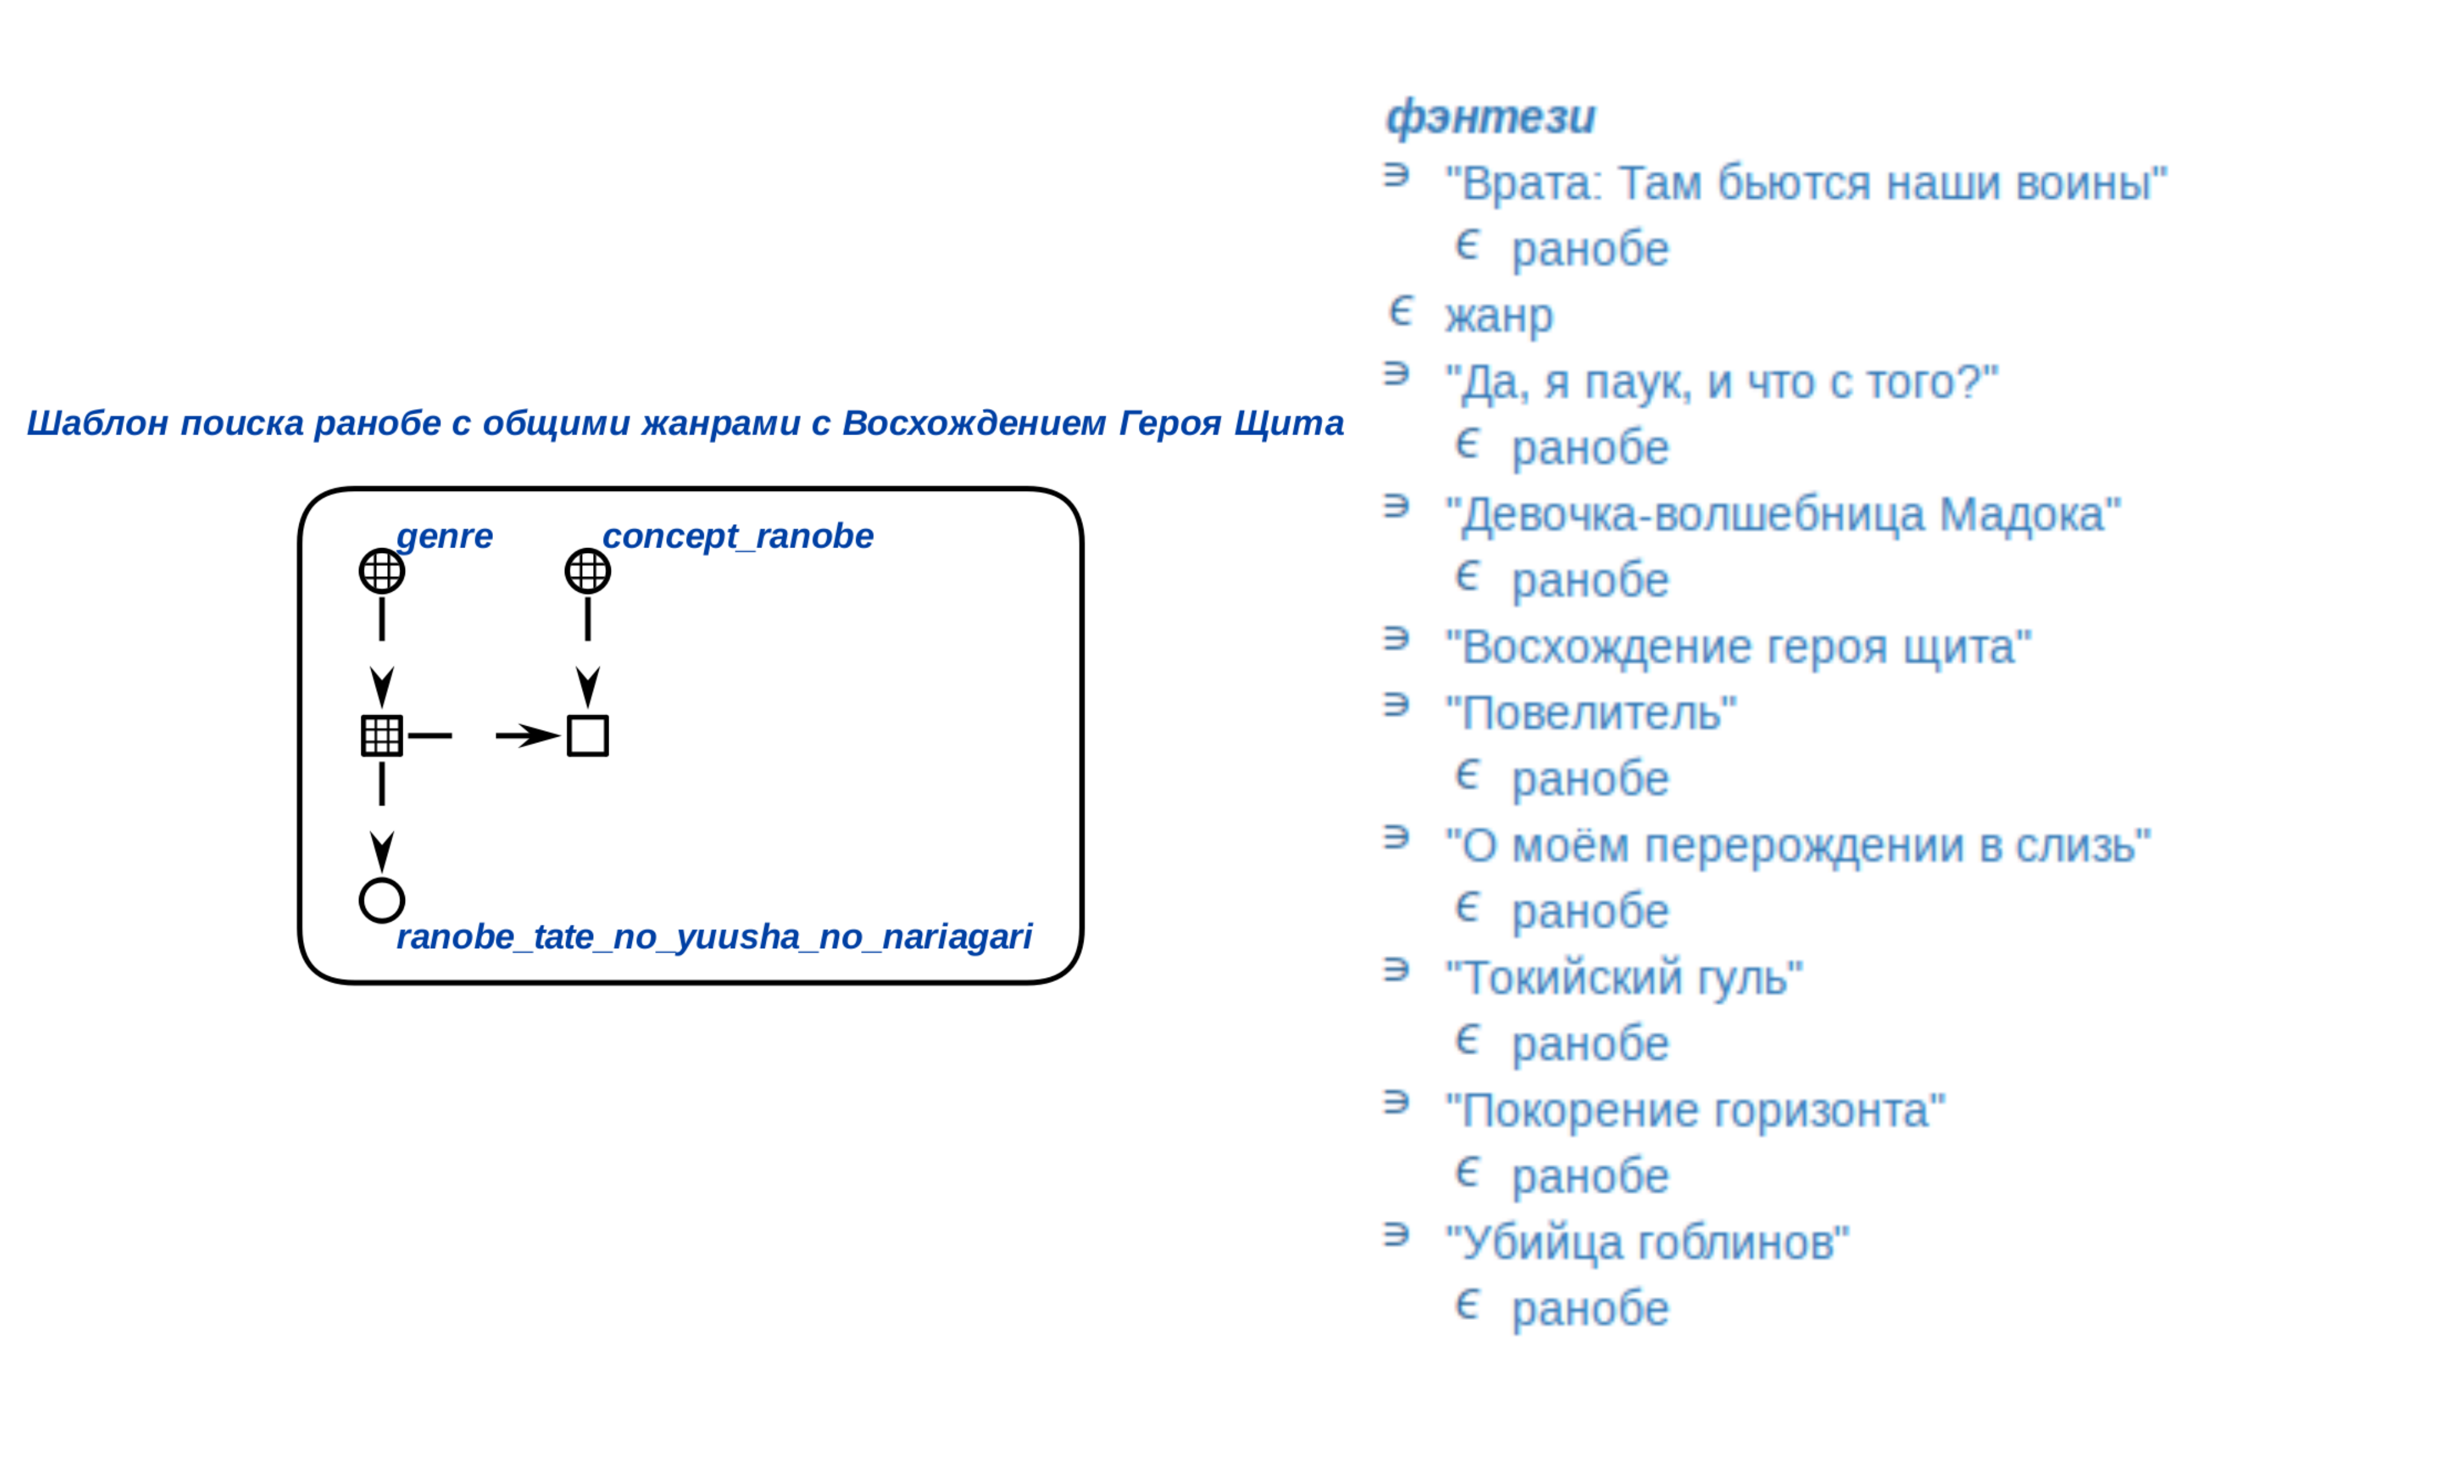
\includegraphics[scale=0.14]{imgs/same_genres.png}
    \caption{Запрос и результат поиска ранобе, имеющих общие жанры с Восхождением Героя Щита}
    \label{fig:search_same_genres}
\end{figure}

\subsection{Вывод}
В результате курсового проектирования был разработан фрагмент базы знаний интеллектуальной справочной системы по библиографии, а именно предметная область японского литературного направления и её частная предметная область -- предметная область ранобе. Раздел отвечает всем требованиям и решает весь перечень задач, поставленных перед ним, а именно:
\begin{itemize}
    \item определена иерархия предметных областей в разработанном фрагменте базы знаний;
    \item для предметных областей определены максимальные и немаксимальные классы исследований, исследуемые отношения, ключевые элементы;
    \item определены необходимые абсолютные и относительные понятия, входящие в предметную область японского литературного направления и ранобе;
    \item приведены формальные описания конкретных сущностей (ранобе, персонажи, авторы, иллюстраторы, жанры, концепции и т.д.).
\end{itemize}

Всего в рамках курсовой работы было разработано более 170 сущностей, которые включают в себя 15 ранобе, 30 авторов и иллюстраторов, 115 персонажей, 5 жанров, 2 популярные в ранобе концепции, а также предметная область ранобе.